\documentclass[11pt,a4paper,twocolumn]{article}
% این فایل و فایلهای ضمیمه‌ی آن از سایت www.parsilatex.com قابل برداشت هستند.
\usepackage{setspace}
\usepackage{subfigure}
\usepackage{algorithm}
\usepackage{algorithmic}
\usepackage{graphicx}
\usepackage{amsmath}
\usepackage[colorlinks, linkcolor=black, citecolor=blue]{hyperref}

\usepackage[top=25mm, bottom=25mm, left=20mm, right=20mm]{geometry}
\setlength{\columnwidth}{82mm}
\setlength{\columnsep}{6mm}

\usepackage{xepersian}
\settextfont[Scale=1]{XB Niloofar}
\setlatintextfont[Scale=.9]{Times New Roman}
\setdigitfont{XB Zar}

\setiranicfont[Scale=.9]{XB Zar Oblique}
\defpersianfont\TitleBold[Scale=1]{XB Niloofar Bold}
\defpersianfont\AbstractBold[Scale=.92]{XB Niloofar Bold}

\renewcommand{\abstractname}{}

% اختصاص - به عنوان جداکننده شماره بخش و زیربخش
\SepMark{-}

% به صورت پیش‌فرض بعد از شماره بخش - نداریم، مگر آنکه شماره زیر بخش پس از آن آمده باشد. از آنجا که مطابق قالب کنفرانس در هر صورت
% پس از شماره بخش و شماره زیربخش به جداکننده نیاز داریم از دستورات زیر استفاده می‌کنیم:
\makeatletter
\renewcommand \thesection {\@arabic\c@section\@SepMark}
\renewcommand \thesubsection {\thesection\@arabic\c@subsection\@SepMark}
\renewcommand \thesubsubsection {\thesubsection\@arabic\c@subsubsection\@SepMark}
\makeatother

% تغییر نام algorithm به الگوریتم
\floatname{algorithm}{الگوریتم}

%\numberwithin{table}{section}
\onehalfspacing

\newcommand\femph[1]{\lr{''}#1\lr{``}}
\newcommand{\SR}{وضوحِ برتر }%{\textiranic{ وضوحِ برتر }}
\newcommand{\HR}{وضوح بالا }
\newcommand{\registration}{ثبت تصویر }
\newcommand{\fusion}{آمیختن }
\newcommand{\fused}{آمیخته }

\newcommand{\warp}{\mathbf{W}(\mathbf{x};\mathbf{p})}
\newcommand{\IWarp}{I(\mathbf{W}(\mathbf{x};\mathbf{p}))}
\newcommand{\round}[2]{\frac{\partial{#1}}{\partial{#2}}}
\newcommand{\roundB}[2]{\frac{\partial{\mathbf{#1}}}{\partial{\mathbf{#2}}}}

\DeclareMathSizes{10.95}{9.2}{7.3}{5.5} %12,10,8,6

\thispagestyle{empty}

% برای اینکه چکیده حاشیه نداشته باشد
\renewcommand\abstract{}

%\expandafter\renewcommand\csname lr\endcsname[2][]{\LR{\resetlatinfont#2}}
%\newcommand{\latinindex}[1]{\index{\lr{#1}}}


\begin{document}
\title{
%\vspace{13mm} برای مطابقت با استیل کنفرانس این خط باید از حالت توضیح خارج شود.
\TitleBold{مروری بر الگوریتم‌های شبکه‌ی عصبی}}
\author{فرزاد عبدالحسینی، سید سبحان میریوسفی، هومن هاشمی\\
دانشگاه صنعتی شریف، دانشکده مهندسی کامپیوتر\\
\lr{\small\{abdolhosseini, miryoosefi, hohashemi\}@ce.sharif.edu}
}
% برخی دستورات زیر برای آن گذاشته شده‌اند که چکیده به صورت تک ستونی باشد
\twocolumn[
\begin{@twocolumnfalse}
\date{}
\maketitle

\begin{abstract}
\AbstractBold
{
\vspace{-5mm}
چکیده - در این مقاله قرار است نگاهی به الگوریتم‌های شبکه‌های عصبی، تاریخچه و کار‌های انجام شده در آن داشته باشیم. با مفاهیم پایه‌ای آن آشنا شده و الگوریتم‌ها و روش‌های به کار رفته را به طور اجمالی بررسی کنیم. فرض شده که مخاطب آشنایی زیادی با این رشته ندارد و بیشتر می‌خواهد یک دید اولیه از آن به دست آورد.
در ابتدا مفاهیم اولیه مورد نیاز همانند تعریف مدل نورون آمده و سپس به بررسی انواع معماری‌های شبکه‌های عصبی پرداخته می‌شود. بعد از آن الگوریتم‌های مختلف یادگیری تا حدی بررسی شده و در انتها بعضی از کاربرد‌های مهم عملی این شبکه‌ها نشان‌داده شده است.

}
 \end{abstract}
{کلید واژه‌ها}- الگوریتم، هوش مصنوعی، شبکه‌های عصبی.\\
\end{@twocolumnfalse}]
% حذف شماره صفحات
%\thispagestyle{empty}
%\pagestyle{empty}
\section{مقدمه}
کار بر روی
\textbf{شبکه های عصبی مصنوعی}
یا به اختصار
\textbf{شبکه های عصبی}
از جایی آغاز شد که دانشمندان به این مهم دست یافتند که سیستم پردازش مغز انسان بسیار متفاوت با سیستم های کامپیوتری دیجیتال مرسوم میباشد. مغز انسان از یک ساختار بسیار پیچیده, غیر خطی و موازی بهره میبرد و همچنین قابلیت بهبود و ارتقای خود را نیز دارا میباشد.

برای مثال قدرت بینایی و بصری انسان را در نظر بگیرید که یک نوع پردازش اطلاعات است. ما اطلاعات رو از محیط بیرون توسط حسگر پیچیده چشم دریافت میکنیم آن هارا تجزیه و تحلیل میکنیم تا بتوانیم چیز هایی که برای تعامل با محیط نیاز داریم بدست آوریم. مغز انسان میتواند فرآیند تشخیص چهره در یک محیط نا آشنا را در کمتر از 200 میلی‌ثانیه انجام دهد در صورتی که فرآیند های بسیار ساده تر از این برای کامپیوتر های حال حاضر چند روز زمان میبرد.

به عنوان مثالی دیگر خفاش را در نظر بگیرید. این خفاش از یک سیستم ردیاب صوتی یا همان سونار بهره میبرد به این شکل که هنگامی که در تعقیب شکار خود است یک موج صوتی از خود ساتع میکند و از روی انکعاس آن توسط طعمه میتواند اطلاعاتی نظیر  سرعت نسبی طعمه, اندازه طعمه و ... بدست آورد. تمام این پردازش های پیچیده در مغز کوچک خفاش که به اندازه‌‌ی یک آلو است انجام می‌پذیرد.

اما مغز انسان یا خفاش چگونه این کار هارا انجام می‌دهد ؟ 
\section{آشنایی و مفاهیم اولیه}
در اینجا ابتدا یک تعریف ارائه میکنیم\cite{haykin}
و سپس در بخش های بعد به توضیح آن میپردازیم:

\textbf{ شبکه عصبی مصنوعی یک پردازنده توزیع شده موازی و گسترده است و که از واحد های پردازشی ساده ساخته شده است که میتواند دانش اکتسابی را در خود دخیره کند و در آینده از آن ها در تصمیم‌گیری ها استفاده کند  از دو جهت این شبکه عصبی مصنوعی  مغز انسان  را تداعی میکند:
}
\begin{enumerate}
\item 
\textbf{اطلاعات از محیط و توسط فرآیند یادگیری کسب میشود.}
 
\item
\textbf{میزان قدرت اتصالات بین واحد های پردازشی(نورون ها) که به آن وزن سیناپسی میگوییم برای دخیره اطلاعات استفاده میشود.}
\end{enumerate}

\subsection{مزایای شبکه های عصبی}
شبکه عصبی قدرت محاسباتی‌اش را از دو ویژگی بهره میگیرد ویژگی اول اینکه یک شبکه بسیار گسترده, موازی و توزیع شده است و ویژگی دوم اینکه قابلیت یادگیری است اینکه میتواند با توجه به محیط یک سری اطلاعات و تجارب کسب کند و از این تجارب در تصمیمگیری های بعدی استفاده کند به این ویژگی
\textbf{کلیت‌بخشی}\LTRfootnote{Generalization}
میگوییم. این ویژگی ها باعث میشود  مسائلی که در حال حاضر برای کامپیوتر های مرسوم دست‌نیافتی است توسط این شبکه ها قابل حل باشد البته باید توجه داشت که گونه های خاصی از مسائل هستند که توسط این شبکه های عصبی به طور بهینه قابل حل هستند و پردازنده  های مرسوم در بعضی موارد بهتر عمل میکنند. باید توجه داشت بخش های مربوط از یک مسئله را توسط این شبکه ها حل کنیم. همچنین تا ساختن شبکه عصبی که به طور کامل مغز انسان یا هر شبکه عصبی طبیعی دیگر را تداعی کند راه طولانی‌ای در پیش داریم.

حالا بعضی از مزایا و توانایی های شبکه های عصبی را ذکر میکنیم:

\begin{itemize}
  \item 
\textbf{توانایی غیرخطی بودن:}\LTRfootnote{Nonlinearity}
  واحد های سازنده شبکه عصبی یا همان نورون ها میتوانند غیرخطی باشند و درنتیجه کل شبکه عصبی غیرخطی میشود این ویژگی بسیار مهم است زیرا بسیاری از مسائل ذاتا غیرخطی هستند مانند پردازش گفتار.
  \item
\textbf{نگاشت ورودی-خروجی:}\LTRfootnote{Input-Output Mapping}
در بسیاری از مسائل ما ارتباط منظقی بین ورودی و خروجی را نمیدانیم ولی برای چند نمونه خاص ورودی خروجی مورد انتظار را در دست داریم ما میتوانیم به کمک این ها شبکه عصبی را آموزش دهیم در اینصورت شبکه عصبی وزن های سیناپسی خود را به گونه‌ای تغییر میدهد که جواب تاحدممکن به خروجی مورد نظر نزدیک شود در اینصورت به گونه ای توانستیم بدون هیچ دانسته قبلی بین ورودی و خروجی های درست نگاشت برقرار کنیم حال میتوانیم از شبکه عصبی برای بدست آوردن خروجی مورد نظر برای ورودی های دیگر استفاده کنیم این تکنینک در مسائل الگویابی بسیار استفاده میشود.
\item
\textbf{تطبیق‌پذیری:}\LTRfootnote{Adaptivity}
ساختار شبکه عصبی به نحوی است که میتواند  خود را در محیط وفق دهد به اینگونه که اگر محیط تغییر کند شبکه عصبی وزن های سیناپسی خود را به گونه این تغییر میدهد که با محیط تغییر یافته تطبیق پیدا کند البته باید توجه داشت که شبکه عصبی نباید بیش از حد هم نسبت به تغییرات حساس باشد زیرا که تغییرات خیلی کوچک که حتی میتواند ناشی از خطای حسگر ها باشد بروی آن تاثیر میگذارد این تطبیق پذیری باید به گونه ای باشد که نه خیلی حساس باشد که پایداری سیستم به هم بریزد نه خیلی بی تفاوت که روند یادگیری و بهبود را مختل کند.
\item
\textbf{تحمل خطا:}\LTRfootnote{Fault Tolerance}
ساختار شبکه های عصبی به علت گستردگی به گونه ایست تحمل خطا و خرابی بالایی دارد . برای مثال با از کار افتادن یک نورون تغییر محسوسی در نتیجه حاصل نیمشود و آسیب باید خیلی زیاد باشد تا کار شبکه را مختل کند.
\item
\textbf{آزمایشات زیستی:}\LTRfootnote{Neurobiological Analogy}
از آن جایی که شبکه عصبی تا حد خوبی میتواند شبکه های عصبی واقعی را تداعی کند از آن میتواند در آزمایشات و پژوهش های زیستی استفاده کرد.
\end{itemize}

\subsection{بررسی مغز انسان}
از آن جایی که شبکه عصبی برگرفته از مغز انسان است ابتدا به بررسی آن میپردازیم . شبکه عصبی مغز انسان یک سیستم سه بخشی است همانطور که در شکل
\ref{fig:three-parts}
نشان داده شده است.

\begin{figure}
  \centering
    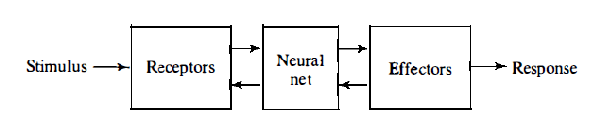
\includegraphics[width=0.4\textwidth]{three-parts.png}
  \caption{ساختار سه بخشی شبکه عصبی انسان}
  \label{fig:three-parts}
\end{figure}
بخش مرکزی همان شبکه عصبی است که شامل شبکه گسترده نورون ها است و محل تصمیم گیری میباشد . بخش اول یا همان گیرنده ها اطلاعات را از محیط گرفته و به سیگنال های قابل فهم برای شبکه عصبی تبدیل میکند و بخش آخر نیز دستورات را از شبکه عصبی گرفته و واکنش موردنظر را در محیط انجام میدهد.

در سال 1911 ساختار نورونی 
\LTRfootnote{Ramon y Cajal}
برای مغز معرفی شد.  نورون ها 5 الی 6 مرتبه توانی از سیلیکون کند تر هستند. اتفاقات در چیپ های سیلیکونی هر 1 نانوثانیه اتفاق میافتد و این در حالی است که در نورون هر 1 میلی‌‌ثانیه . ولی مغز انسان این سرعت کم نورون ها را  با تعداد بسیار زیاد آن ها و اتصلات(سیناپس ها) بسیار زیادتر جبران کرده است. تخمین زده میشود که تعداد نورون ها حدود 10 میلیارد و تعداد اتصلات بین آن ها حدود 60 تریلیارد است. از طرفی دیگر مصرف انرژی مغز انسان در مقایسه با چیپ های سیلیکونی حدود 10 مرتبه توانی کمتر است. در شکل
\ref{fig:bio-neuron}
ساختار نورون و سیناپس را مشاهده میکنید.

\begin{figure}
  \centering
    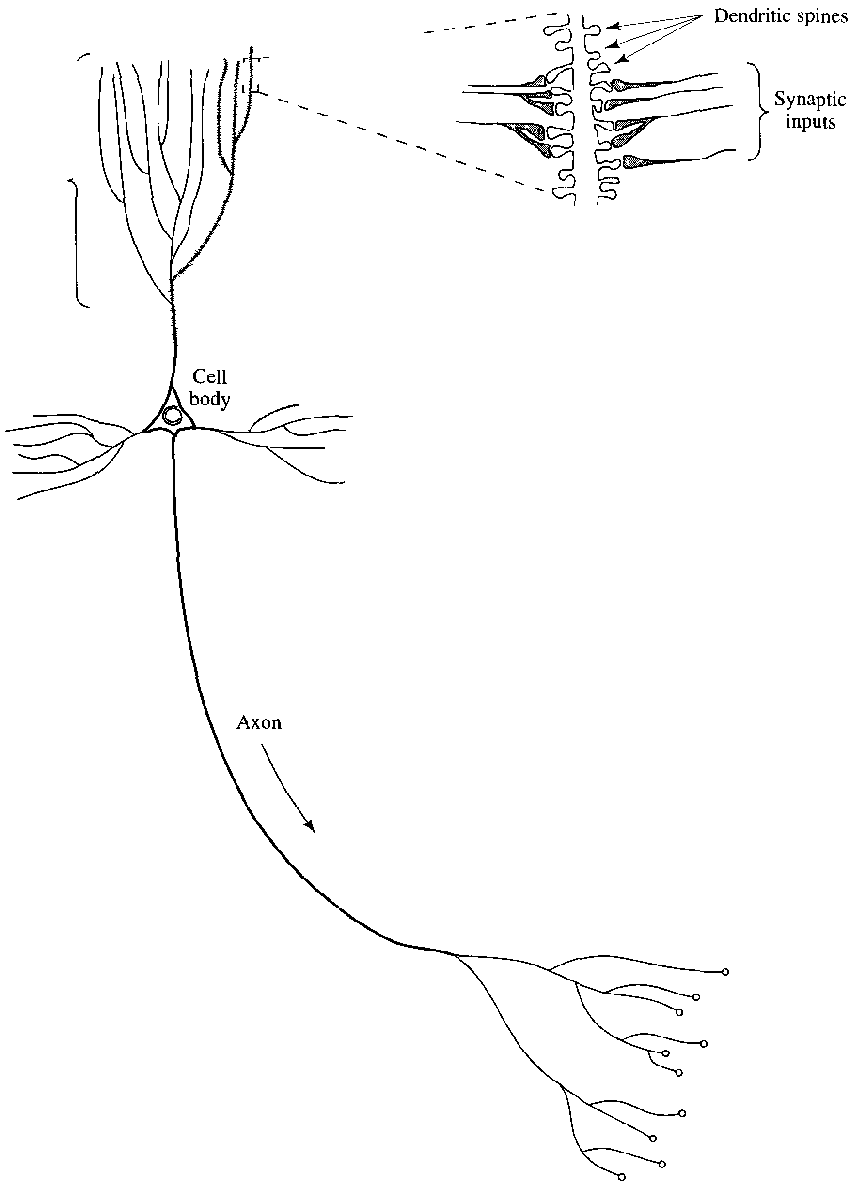
\includegraphics[width=0.45\textwidth, height=0.5\textwidth]{bio-neuron.png}
  \caption{ساختار نورون زیستی}
  \label{fig:bio-neuron}
\end{figure}


\subsection{مدل نورون برای شبکه عصبی}
	نورون یک واحد پردازش اطلاعات است که واحد سازنده شبکه عصبی است در شکل 3 مدل ارائه شده برای نورون را مشاهده می‌کنید . در اینجا به تشریح بخش های مختلف می پردازیم:
\begin{itemize}
\item
\textbf{سیناپس ها یا اتصالات}
هر کدام به همراه یک عدد که به آن وزن سیناپسی میگوییم مشخص شده اند هنگامی که سیگنال
$x_i$
را در سیناپس
$j$
از نورون
$k$
داشته باشیم و وزن سیناپسی این سیناپس
$W_{k,j}$
باشد آن وقت سیگنال ورودی در وزن سیناپسی ضرب میشود.
\item
یک \textbf{جمع کننده}  که مقادیر ورودی (سیگنال های ضرب شده در وزن سیناپسی) و همچنین مقدار ثابت (\lr{bias}) را جمع می کند.
\item
\textbf{تابع فعال سازی}
که مقدار حاصل جمع را میگیرد و خروجی مورد نظر را تولید میکند.	
\end{itemize}

\begin{figure}
  \centering
    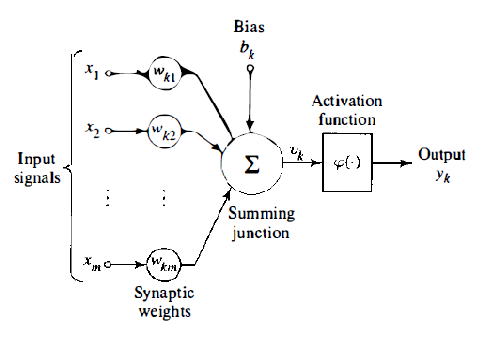
\includegraphics[width=0.4\textwidth]{neuron.png}
  \caption{مدل ریاضی ارائه شده برای نورون}
  \label{fig:neuron}
\end{figure}

همانطور که در بالا توضیح دادیم داریم:
$$u_k = \sum_{j=1}^{k}{W_{k,j}X_j}$$
$$v_k = u_k + b_k$$
$$y_k = \varphi(v_k)$$
به مقدار $v_k$ در عبارت بالا
\textbf{پتانسیل فعالسازی}
نورون می‌گوییم.

\subsection{انواع توابع فعال‌سازی}
\label{sec:activation}

\begin{itemize}
\item
\textbf{تابع \lr{Threshold}}:
این تابع به نوعی بر اساس اینکه مقدار ورودی میزان مشخصی را رد کرده است یا خیر تصمیم گیری انجام می دهد و بسیار پر کاربرد است:
\[ \varphi(v) =
  \begin{cases}
    1\quad \text{if}\quad v \ge 0\\
    0\quad \text{if}\quad v < 0 \\
  \end{cases}
\]
\item
\textbf{تابع \lr{PicewiseLinear}}:
این تابع حالت بسیار تیز تغییر تصمیم در مدل قبلی را به کمک تابعی خطی بهبود بخشیده است:
\[ \varphi(v) =
  \begin{cases}
    1\quad\quad\;\;\;\text{if}\quad v > \frac{1}{2}\\
    v+\frac{1}{2}\quad \text{if}\quad -\frac{1}{2} \le v \le \frac{1}{2} \\
    0\quad\quad\;\;\;\text{if}\quad v < -\frac{1}{2}\\
  \end{cases}
\]

\item
\textbf{تابع \lr{Sigmoid}}:
این تابع یکی از پرکاربردترین توابع فعال سازی است در واقع چیزی بین دو حالت قبلی است. توجه کنید اگر ثابت $a$ را به سمت بینهایت میل بدهیم تبدیل به تابع
\lr{Treshold}
می‌شود.
$$\varphi(v) = \frac{1}{1+\exp(-av)} $$

\item
\textbf{مدل احتمالاتی}:
در بعضی از مسائل نیاز است که تابع فعال سازی ما تصمیم قطعی نگیرد و به صورت احتمالاتی عمل کند مانند مثال زیر:
$$P	(v) = \frac{1}{1+\exp(-av)} $$
\[ \varphi(v) =
  \begin{cases}
    +1 \quad \text{\lr{with probability}} \quad P(v)\\
    -1 \quad \text{\lr{with probability}} \quad 1-P(v)\\
  \end{cases}
\]


\end{itemize}

\subsection{نمایش شبکه عصبی با گراف جهتدار}
 شبکه عصبی را میتوان به وسیله یک گراف جهتدار نشان داد . این گراف از سه قاعده زیر طبعیت میکند:
 
\begin{itemize}
	\item
\textbf{قاعده 1:}
سیگنال در جهت یال منتقل میشود  2 نوع یال در گراف موجود است:
\begin{itemize}
	\item
\textbf{یال سیناپسی:}
در این یال مقدار ورودی یال (سیگنال گره‌ی ابتدای یال) در وزن نوشته شده روی یال که در واقع همان وزن سیناپسی است ضرب میشود تا حاصل تولید شود.
\item
\textbf{یال فعال‌سازی:}
در این یال مقدار ورودی یال یال (سیگنال گره‌ی ابتدای یال) به عنوان ورودی تابع نوشته شده روی یال در نظر گرفته میشود تا حاصل تولید شود.
\end{itemize}
\item
\textbf{قاعده 2:}
سیگنال یک گره جمع جبری سیگنال یال هایی است که به آن وارد میشوند.
\item
\textbf{قاعده 3:}
یال هایی که از یک گره خارج میشوند از هم مستقل بوده و سیگنال اولیه برابر سیگنال گره دارند.
\end{itemize}
در شکل
\ref{fig:type-1}
و
\ref{fig:type-2}
میتوایند این سه قاعده را مشاهده کنید.	
\begin{figure}
  \centering
    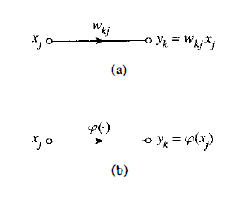
\includegraphics[width=0.4\textwidth]{type-1.png}
  \caption{قاعده‌ ۱}
  \label{fig:type-1}
\end{figure}

\begin{figure}
  \centering
    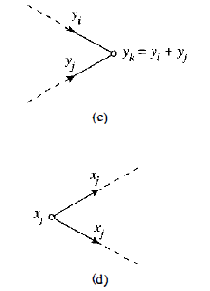
\includegraphics[width=0.4\textwidth]{type-2.png}
  \caption{قاعده ۲ و ۳}
  \label{fig:type-2}
\end{figure}
در نتیجه میتوانیم تعریفی دیگر\cite{haykin}
 برای شبکه عصبی ارائه دهیم:
\\

\textbf{شبکه عصبی یک گراف جهتدار است تشکیل شده از گره و یال هی سیناپسی یا فعال‌سازی و دارای چهار ویژگی زیر است:
}
\begin{itemize}
\item\textbf{
هر نورون متشکل از تعدادی یال سیناپسی و حداکثر یک یال فعال‌سازی است.}
\item\textbf{
وزن یال های سیناپسی نشان دهنده وزن های سیناپسی است (مقادیر قابل تغییر در یادگیری).}
\item\textbf{
جمع سیگنال یال های سیناپسی پتانسیل فعال سازی گره را میسازد.}
\item\textbf{
تابع فعال سازی روی پتانسیل فعال‌سازی اعمال میشود و خروجی نورون تولید میشود.}
\end{itemize}
در شکل
\ref{fig:neuron-graph}
میتوانید مدل نورون ارائه شده را به عنوان یک گراف جهتدار مشاهده کنید.
\begin{figure}
  \centering
    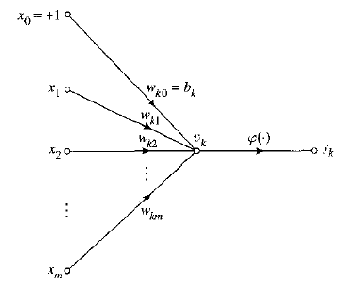
\includegraphics[width=0.4\textwidth]{neuron-graph.png}
  \caption{مدل گراف جهتدار برای نورون}
  \label{fig:neuron-graph}
\end{figure}

\subsection{معماری شبکه عصبی}
به نحوه قرار گرفتن گره در شبکه عصبی و اتصلات بین آن ها معماری شبکه عصبی می گویند. معماری شبکه‌های عصبی را به چند دسته‌ی اصلی تقسیم می‌کنیم:

\begin{enumerate}
\item
\textbf{شبکه های رو به جلو:}
شبکه هایی که در ساختار گراف آن ها دور وجود ندارد. 
\begin{itemize}
\item
\textbf{شبکه های تک لایه:}
شبکه های رو به جلویی که تنها شامل دو سطح از گره هستند سطح گره ورودی و سطح گره خروجی(نورون های خروجی).
\item
\textbf{شبکه های چند لایه:}
شبکه هایی که حداقل دارای یک سطح بیشتر از شبکه های تک لایه هستند. ( به لایه های میانی لایه های پنهان نورون نیز میگویند)
\end{itemize}
\item
\textbf{شبکه های درجریان:}
شبکه هایی که در ساختار گراف ان ها دور وجود دارد.
\end{enumerate}


\section{الگو‌های اتصالات}
در بخش قبل، دسته‌بندی انواع معماری‌های مختلف در شبکه‌های عصبی انجام شد. در این بخش می‌‌خواهیم این دسته‌بندی‌ها را به تفصیل بررسی کنیم.

در بین معماری‌های مختلف، ساده‌ترین‌شان شبکه‌های تک لایه‌ی رو به جلو و پر قدرت‌ترین‌شان شبکه‌های در جریان اند. اما به دلیل آن که برای این نوع شبکه‌ها به صورت کلی هنوز الگوریتم‌های یادگیری کارآمدی طراحی نشده، از آن‌ها کمتر استفاده می‌شود و در نتیجه پرکاربرد‌ترین معماری، همان شبکه‌های چند لایه‌ی رو به جلو اند که هم توانایی بسیار بالایی دارند و هم توانایی یادگیری بالا.

البته انواع مختلفی از شبکه‌های در جریان خاص ساخته شده‌اند که الگوریتم‌های یادگیری خوبی نیز دارند و در موضوعاتی که مورد استفاده قرار گرفته‌اند قدرت بالایی از خود نشان داده‌اند. اما هنوز اگر الگوریتم مناسبی برای حالت کلی شبکه‌های در جریان پیدا شود، می‌تواند باعث پیشرفت بزرگی بشود.

در واقع همانطور که در بخش
\ref{sec:single-neuron}
نشان داده می‌شود، می‌توان با استفاده از نرون‌های بسیار ساده، تمام گیت‌های پایه‌ای یک رایانه را پیاده‌‌سازی کرد، پس قدرت محاسبه‌ای شبکه‌های عصبی مصنوعی حداقل به اندازه‌ی قدرت رایانه‌ها است (حداقل در تئوری) با این تفاوت که قدرت اصلی این شبکه‌ها در قابلیت یادگیری آن‌ها بدون کمک برنامه‌ریزی از قبل و دانستن مسئله‌های پیش رو است.

شبکه‌های عصبی را شاید بتوان همانند با سلول‌های بنیادی در نظر گرفت که می‌توانند بدون این که برای کاری اختصاصی شده باشند، آن‌ها را در محیط قرار دهیم و خود به خود، خودشان را با محیط تطبیق دهند و کار را به خوبی انجام دهند.
\subsection{شبکه‌های تغذیه‌ی رو به جلو}
ساده‌ترین نوع شبکه‌های عصبی،‌ شبکه‌هایی اند که در ساختارشان دور وجود نداشته باشد. یعنی خروجی یک گره هرگز (بعد از یک یا چند مرحله) به خود آن گره برنگردد. در نتیجه اطلاعات همیشه از یک قسمت وارد شده و بعد از گذشتن از درون یک یا چند نورون‌ مختلف به انتهای مسیر (گره‌های خروجی)‌ می‌رسند. معمولا این شبکه ها را در حالت کلی به صورت شکل 
\ref{fig:multilayer}
نشان می‌دهند.

اهمیت این معماری ساده در این است که با وجود سادگی،‌ توانایی بالایی دارند و مهم‌تر از آن، برای آن‌ها الگوریتم‌های یادگیری کارآمد وجود دارد. در مقابل، معماری‌های پیچیده‌تری که جلو‌تر خواهیم دید، با وجود پتانسیل بالا نمی‌توانند از قدرت خود به حد کافی استفاده کنند (به جز در مواردی که برای یک دسته سوال اختصاصی شده‌اند).

\subsection{شبکه‌های تک لایه}
این نوع از شبکه‌های رو به جلو همانطور که از اسم‌شان مشخص است، فقط یک لایه نورون دارند (البته اگر گره‌های ورودی را نورون فرض نکنیم) و از آن‌ها با نام 
پرسپترون\LTRfootnote{perceptron}
یاد می‌شود. این شبکه‌ها در سال ۱۹۶۰ توسط
فرانک روزنبلت\LTRfootnote{Frank Rosenblatt}
در دنباله‌ای از مقالات و یک 
کتاب\LTRfootnote{Principles of Neurodynamics: Perceptrons and the Theory of Brain Mechanisms, Spartan Books, 1962}
بررسی شده و توسعه داده‌ شدند. پس از انتشار این کتاب، شبکه‌های تک لایه محبوبیت زیادی به دست‌آوردند و نویسنده محبوبیت جهانی به دست آورد. پس از آن تحقیقات زیادی بر روی این شبکه‌ها انجام شد و محققان اکثرا انتظارات بسیار زیادی از آن‌ها داشتند تا این که مینسکی\LTRfootnote{Marvin Minsky}
و پپرت\LTRfootnote{Seymour Paper}
در کتاب‌شان با نام پرسپترون
\LTRfootnote{Perceptrons: an introduction to computational geometry, 1969}
در سال ۱۹۶۹ با نشان دادن محدودیت‌های این نوع شبکه‌ها، از شور و هیجان این تحقیقات به طور قابل ملاحظه‌ای کاستند تا حدی که تا سال ۱۹۸۰ تقریبا تحقیق بر روی این شبکه‌ها متوقف شد.\cite{wiki-frank}

یک مثال قابل توجه از بزرگنمایی‌هایی که در مورد توانایی پرسپترون‌ها قبل از انتشار مقاله‌ی مینسکی و پپرت انجام گرفت، پروژه‌ای بود که در آن تعدادی عکس که در هر کدام دقیقا یک تراکتور یا یک تانک (در محیط‌های مختلف) قرار داشت به یک شبکه‌ی عصبی داده شد و هدف این بود که این شبکه بتواند در نهایت تشخیص بدهد که وسیله‌ی موجود در عکس تانک بوده یا تراکتور. حتی در بعضی از این عکس‌ها قسمتی از وسیله توسط درختان جنگلی پوشیده شده بود و وسیله به طور کامل دیده نمی‌شد. این پروژه در ابتدا نتایج بسیار موفقیت آمیزی داشت و به خوبی می‌توانست بین دو وسیله تشخیص درست بدهد. اما در نهایت مشخص شد که دلیل نتایج درست این شبکه این بوده که عکس تراکتورها در یک روز آفتابی و عکس تانک‌ها در یک روز ابری گرفته شده بود و تنها کاری که شبکه انجام می‌داد تعیین مقدار روشنایی تصویر و تصمیم‌گیری بر اساس آن بود، کاری که برای چشم انسان (حداقل با دقت بالا) کار ساده‌ای نیست، اما برای نورون ها به سادگی قابل انجام است. اینگونه اتفاقات می‌توانند یک الگوریتم را به سرعت بدنام کنند.	\cite{ml-hinton}

ساده‌ترین مثالی که شبکه‌های تک لایه در شبیه‌سازی‌شان عاجز اند، گیت منطقی 
\lr{xor}
 است. البته این تنها مثال نیست و فقط نماینده‌ی گروه بزرگی از توابع است که نورون‌ها قابلیت تولید خروجی همانند‌شان را ندارند، اما خبر خوب این است که این مشکل با اضافه کردن تعداد لایه‌ها حل می‌شود و همین گیت 
 \lr{xor}
 با دو لایه نورون به سادگی قابل پیاده‌سازی است.
 
یک نکته‌ي مهم درتحلیل و بررسی رفتار شبکه‌های تک لایه این است که اگر دقت کنید، هر کدام از نورون‌ها کاملا به طور مستقل از دیگر نورون‌ها رفتار می‌کند چون مقادیر ورودی را که نمی‌توانیم تغییری بدهیم و بین نورون‌های سطح اول هم هیچ ارتباطی وجود ندارد. پس برای مثال هر شبکه‌ی تک لایه با $k$ نورون را می‌توان $k$ تا شبکه با فقط یک نورون در نظر گرفت که البته ورودی تمام‌شان را یکی می‌دهیم. این موضوع باعث می‌شود که تحلیل این شبکه‌ها بسیار ساده باشد و الگوریتم یادگیری کارایی برای آن‌ها طراحی شود. البته این موضوع باعث می‌‌شود که به سادگی ببینیم که این نوع شبکه‌ها توانایی بالایی در حل مسائل مختلف ندارند و با بزرگ‌تر کردن‌شان بر قدرت‌شان افزوده نمی‌شود.

\subsubsection{مثال‌هایی از قدرت تک نورون}
برای نشان دادن حداقل توانایی های یک نورون ساده، با استفاده از آن‌ها گیت‌های منطقی پایه‌ای رایانه و دو مثال پیشرفته‌تر را طراحی می‌کنیم. برای این کار فرض کنید که تابع فعال‌سازی تمام نورون‌های این بخش و بخش بعد از نوع تابع 
\lr{Threshold}
(که در بخش
\ref{sec:activation}
تعریف شده) می‌باشد:
\begin{itemize}
  \item
\textbf{گیت \lr{not}:}
برای ساختن این گیت باید یک ورودی داشته باشیم که ضریب آن را برابر $-1$ قرار می‌دهیم و  مقدار عدد ثابت (\lr{bias}) را برابر $0$ قرار می‌دهیم و یک گیت \lr{not} ساخته می‌شود.
  \item
\textbf{گیت \lr{and}:}
برای ساختن این گیت باید دو ورودی داشته باشیم که ضریب هر کدام را برابر $1$ قرار می‌دهیم و  مقدار عدد ثابت را برابر $1.5$ قرار می‌دهیم. حال مقدار خروجی فقط در صورتی یک است که هر دو ورودی یک باشند.
  \item
\textbf{گیت \lr{or}:}
همانند \lr{and} دو ورودی داریم با ضریب $1$ و فقط  مقدار عدد ثابت را برابر $0.5$ قرار می‌دهیم. حال اگر هر کدام را یک کنیم، جواب یک می‌شود. (در شکل
\ref{fig:linear_separability}
هر دو گیت \lr{and} و \lr{or} نشان داده شده.)
  \item
\textbf{تابع اکثریت}
یعنی این که $n$ ورودی داشته باشیم و بگوید که اکثریت آن‌ها صفر بوده‌اند یا یک: برای این تابع هم $n$ ورودی داریم که ضریب هر کدام یک است و مقدار عدد ثابت برابر 
$-\frac{n}{2}$
است.
  \item
\textbf{فلیپ‌فلاپ\LTRfootnote{flip-flop}:}
\label{sec:single-neuron}
ساخت این قطعه به داشتن دور در گراف ساختار نورون‌ها دارد و در نتیجه فقط در شبکه‌های در جریان (بخش
\ref{sec:recurrent}
)
قابل پیاده‌سازی است. اما برای ساخت آن فقط کافی است که خروجی نورون به عنوان ورودی دوباره به خودش داده شود (با ضریب $1$) و دو سیگنال ورودی \lr{set} با ضریب $1$ و \lr{reset} با ضریب منفی $-2$ (البته بسته به استفاده می‌تواند $-1$ هم باشد) و عدد ثابت (\lr{bias}) هم برابر $-1$ باشد. حال تا وقتی که سیگنالی نیاید، همیشه مقدار خروجی نورون ثابت می‌ماند و با آمدن سیگنال هم مقدار آن تعیین می‌شود.
\end{itemize}

\subsubsection{ناتوانی‌های تک نورون}
برای این که بگوییم یک نورون‌ها نمی‌تواند چه کار‌هایی را انجام دهد، ساده‌تر است که نشان دهیم چه کار‌هایی می‌تواند بکند و هر چه در آن قالب نگنجد، کار‌هایی است که نمی‌تواند انجام دهد. (در این بخش فقط با توابع فعال‌سازی \lr{Treshold} کار می‌کنیم)

فرض کنید نورونی که می‌خواهیم بررسی کنیم $n$ یال ورودی دارد. حال یک فضای $n$ بعدی را در نظر بگیرید که به ازای هر یال ورودی یک بعد دارد. حال هر کدام از نقطه‌های این فضا $n$ بعدی یک حالت از مقادیر ورودی نورون را نشان می‌دهد. حال  کاری که نورون ما باید انجام بدهد این است که به ازای هر نقطه،‌ مشخص کند که خروجی‌اش باید صفر باشد یا یک. حال با مقدار دهی به وزن‌ها (و مقدار ثابت (\lr{biass})) ما در واقع یک ابر صفحه‌ی $n$ بعدی انتخاب می‌کنیم و به نقاطی که در یک طرف صفحه باشند مقدار یک و باقی نقاط مقدار صفر را اختصاص می‌دهیم.\cite{ml-hinton}

با استفاده از این تعریف متوجه می‌شویم که یک نورون فقط در زمانی می‌تواند یک تابع با خروجی صفر و یک را تولید کند که نقاط آن (مثلا فقط نقاطی که خروجی‌شان یک است) خاصیت
جدایی‌پذیری خطی\LTRfootnote{Linear separability}
داشته باشند.

ساده‌ترین تابعی که چنین خاصیتی را ندارد، تابع \lr{xor} است که این موضوع در شکل
\ref{fig:linear_separability}
به خوبی نشان داده شده است.
\begin{figure}
  \centering
    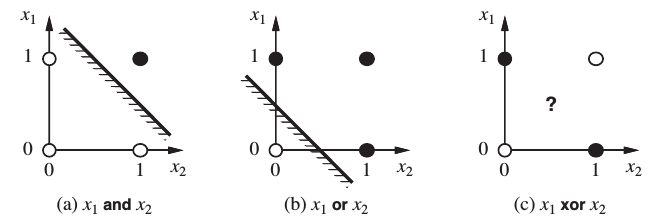
\includegraphics[width=0.4\textwidth]{linear_separability.png}
  \caption{جدایی ناپذیری خطی \lr{xor} (کتاب راسل\cite[ص-۷۳۰]{russell})}
  \label{fig:linear_separability}
\end{figure}

\subsection{شبکه‌های چند لایه}
\label{sec:multilayer}
\begin{figure}
  \centering
    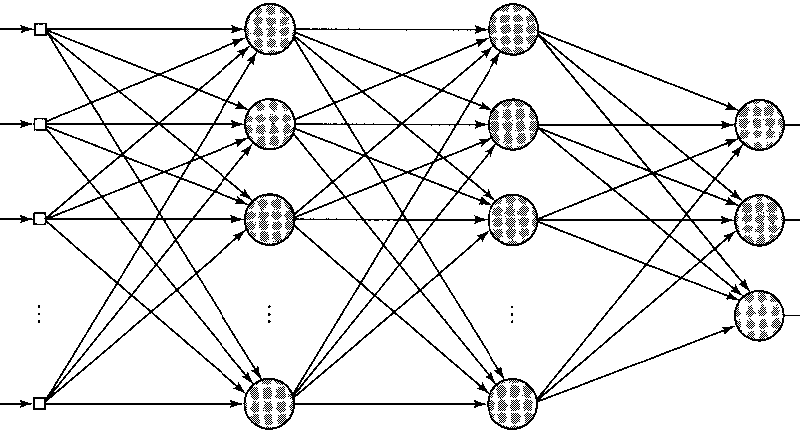
\includegraphics[width=0.4\textwidth]{multilayer.png}
  \caption{ معماری شبکه‌های چند لایه (این مثال: سه لایه)}
  \label{fig:multilayer}
\end{figure}

این شبکه‌ها که حالت کلی شبکه‌های رو به جلو اند، امروزه مدل استاندارد مورد استفاده برای بیشتر مسائل تشخیص الگو با کمک یادگیری با ناظر اند. با ظهور و استفاده از این شبکه‌ها در الگوریتم‌های شبکه‌های عصبی، جان تازه‌ای در تحقیقات در این زمینه دمیده شد. این شبکه‌ها محدودیت‌های شبکه‌های تک لایه در تولید فقط بعضی از انواع توابع خروجی را ندارند.

یکی از مشکلاتی که شبکه‌های تک لایه با آن روبرو بودند این بود که برای این که بهتر کار کنند، نیاز بود که ابتدا از ورودی‌ها چند خاصیت کلی استخراج شوند و سپس با استفاده از این خاصیت‌ها پرسپترون‌ها کار تصمیم گیری را انجام بدهند. اما با استفاده از شبکه‌های چند لایه می‌توانیم ابتدا حتی بدون دانستن خروجی‌ها (بدون ناظر) مقدار زیادی خواص را فقط با داشتن ورودی‌های محتلف از آن‌ها استخراج کنیم و سپس با یا بدون داشتن خروجی‌ها شروع به تصمیم‌گیری کنیم. به همین دلیل این الگوریتم‌ها برای
داده‌کاوی\LTRfootnote{DataMining}
در مجموعه‌ی عظیمی از داده‌ها حتی وقتی که نمی‌دانیم دنبال چه چیزی می‌گردیم و برای مثال فقط می‌خواهیم دنبال بی‌قاعدگی‌ها بگردیم بسیار مناسب هستند. برای اطلاعات بیشتر و کاربرد‌های عملی این شبکه‌ها می‌توانید به ابزار متن‌باز
وکا\LTRfootnote{http://www.cs.waikato.ac.nz/ml/weka/}
مراجعه‌کنید.

در معماری این شبکه‌ها تعدادی لایه نرون وجود دارد که نه گره‌ ورودی‌اند و نه گره‌ خروجی. به این لایه‌ها در اصطلاح،
لایه‌های پنهان\LTRfootnote{hidden layers}
می‌گویند. اهمیت این لایه‌ها در این است که این لایه‌ها تنها چیزی‌اند که شبکه‌های چند لایه را از شبکه‌های تک لایه جدا می‌کنند،‌ پس قدرت این شبکه‌ها بر دوش این لایه‌ها است. اما وجود این لایه‌ها مشکلاتی را برای الگوریتم‌های یادگیری ایجاد می‌کند.

در ادامه بعضی از این مشکلات را بررسی کرده و راه‌حل‌های آن‌ها را ارائه می‌دهیم.

\subsubsection{بیش‌برازش}
بیش‌برازش\LTRfootnote{overfitting} 
به پدیده‌ی نامطلوبی در مدل‌های آماری گفته می‌شود که در آن درجه‌ی آزادی مدل بسیار بیشتر از درجه‌ی آزادی واقعی انتخاب شده و در نتیجه اگرچه مدل روی داده‌های استفاده شده برای یادگیری بسیار خوب نتیجه می‌دهد،‌ اما بر روی داده‌های جدید دارای خطای زیاد است.\cite{wiki-overfitting}
برای مثال وقتی که مقدار یک چند جمله‌ای درجه‌ی دو را با یک چند جمله‌ای درجه‌ی سه تخمین بزنیم.

همانند تمام مدل‌های آماری، شبکه‌های چند لایه نیز وقتی که تعداد پارامترهای مسئله (همان تعداد لایه‌ها و اندازه‌ی کلی شبکه) بیش از حد باشد، به مشکل بیش‌برازش بر می‌خوریم. در این حالت حتی شبکه‌ی ما می‌تواند به صورتی تمام ورودی‌های داده‌شده را در خود ذخیره کند و بر روی آن‌ها درست جواب بدهد اما لزوما این نتایچ را بر روی ورودی‌های جدید تعمیم ندهد.

به وضوح اگر اندازه‌ی شبکه بسیار کوچک باشد نیز
مشکلات دیگری\LTRfootnote{underfittin}
پیش می‌آید و نتایج دقت کافی را ندارند.

اگر قرار باشد در شبکه موجود تمام گره‌ها به یکدیگر وصل باشند، تنها موضوع باقی‌مانده، اندازه‌ی شبکه است. یکی از روش‌های ساده برای حل این مشکل این است که ابتدا چند ساختار را بررسی کنیم و کوچک‌ترین ساختاری را انتخاب کنیم که نتایج قابل قبولی دارد. روش‌های دیگر استفاده از روش
اعتبار‌سنجی متقابل\LTRfootnote{cross-validation}
است. یک روش برای شبکه‌های تماما متصل نیستند، الگوریتم
صدمه‌ی مغزی بهینه\LTRfootnote{optimal brain damage}
است که ابتدا از یک گراف کامل شروع می‌کند و سپس بعضی از ارتباطات آن‌را حذف می‌کند.
\cite[ص-۷۳۷]{russell}

\subsubsection{انتشار رو به عقب}
یکی از ابتدایی ترین مشکلات شبکه‌های چند لایه این است که نیاز به الگوریتم کارایی برای انجام یادگیری در لایه‌های نهفته داریم. به این دلیل که این لایه‌ها به طور مستقیم به خروجی‌ها وصل نیستند و نمی‌توانیم به طور مستقیم خروجی‌شان را بررسی کرده و بر اساس آن تغییرات لازم را انجام بدهیم. یکی از اولین و پرکاربردترین روش‌های ارائه شده، الگوریتم
انتشار رو به عقب\LTRfootnote{back propagation}
است. در این روش مقدار خطای لایه‌های عقب‌تر بر اساس خطای لایه‌های جلو‌تر به دست می‌آید و به اصطلاح خطا رو به عقب انتشار پیدا می‌کند. یک پیش‌نیاز برای انجام این روش این است که توابع فعال‌سازی نورون‌ها توابعی پیوسته باشند. برای مثال می‌توان از تابع فعال‌سازی \lr{Sigmoid}\
(بخش \ref{sec:activation})
استفاده کرد.

برای بهتر فهمیدن روش این الگوریتم، در نظر بگیرید که خروجی نورون‌های لایه‌های جلو‌تر یک تابع بر حسب خروجی نورون‌های لایه‌های مرحله‌ی قبل است. حال با در دست داشتن مقدار خطای‌ تابع می‌توانیم مقدار تاثیر پارامتر‌های ورودی تابع را در خطا محاسبه کنیم. با انجام این کار و انتشار مقدار خطای به دست آمده به مراحل قبل، مقدار خطای آن‌ها نیز به دست می‌آید.\cite{ml-hinton}

یک نکته‌ی مهم در مورد درستی این روش این است که شاید این روش بهترین روش ممکن نباشد، یک الگوریتم کارا هم نظر پردازشی و هم از نظر نتایج به دست آمده است.

اما هنوز این روش نمی‌تواند به عنوان یک روش یادگیری کامل بر روی تمام شبکه‌ها استفاده شود. به شبکه‌‌هایی که تعداد لایه‌های زیادی (در واقع تعداد لایه‌های پنهان زیاد) داشته باشند،
شبکه‌های عمیق\LTRfootnote{deep networks}
می‌گویند. در هنگام اجرای این الگوریتم بر روی این شبکه‌ها دیده می‌شود که یادگیری بعد از چند سطح دیگر کار خود را نمی‌تواند به خوبی انجام دهد. این مشکل به دلیل موضوعی به نام
مسئله‌ی گرادیان محو شونده\LTRfootnote{Vanishing Gradient problem} ایجاد می‌شود. 
یعنی سهم خطایی که برای لایه‌های قبلی محاسبه می‌کردیم، بعد از چند مرحله به سرعت از بین می‌رود و شاید حتی بعد از چهار مرحله، مقدار به دست آمده با تقریب خوبی برابر صفر باشد. به همین دلیل معمولا ابتدا برای لایه‌های اولیه از الگوریتم‌های یادگیری بدون ناظر استفاده می‌شود و سپس برای لایه‌های انتهایی از این الگوریتم یا الگوریتم‌های مشابه استفاده می‌شود.
	
\subsection{شبکه‌های در جریان}
\label{sec:recurrent}
این نوع شبکه‌ها بسیار قدرتمندتر از شبکه‌های رو به جلو اند. در کل در طراحی
شبکه‌های در جریان\LTRfootnote{recurrent}
می‌تواند دور‌های جهت‌دار وجود داشته باشد، یعنی یک داده می‌تواند پس از گذشتن از چند مرحله دوباره به جای اولیه خود برگردد. به همین دلیل این شبکه‌ها توانایی نگه‌داری داده‌ها در طول زمان (عنصر حافظه همانند فلیپ‌فلاپ که در بخش
\ref{sec:single-neuron}
نشان داده شد) را دارند. و همان طور که در بخش مذکور نشان داده شد، می‌توانند تمام اجزای پایه‌ای یک رایانه‌ی کامل را داشته باشند. پس اگر بتوانیم آن‌ها را تعلیم دهیم قدرت بسیار بالایی می‌توانند داشته باشند. اما به دلیل این که می‌توانند اشکال بسیار مختلف و پیچیده‌ای داشته باشند، الگوریتم‌های یادگیری مناسبی برای‌شان به دست نیامده و به همین دلیل در حال حاضر نمی‌توانیم از تمامی قدرت‌شان استفاده کنیم و طراحی چنین الگوریتمی بسیار مورد نیاز و سودمند است.

این شبکه‌ها طبیعی‌ترین روش برای مدل کردن داده‌های پشت سر هم (دنباله‌ی داده‌ها) هستند. معمولا در هنگام عمل یادگیری برای این شبکه‌ها آن‌ها را به صورت شبکه‌های چند لایه‌ی رو به جلو مدل می‌کنیم که در زمان عمق پیدا کرده اند. یعنی برای هر مرحله‌ی زمان، یک بار کل شبکه‌ را قرار می‌دهیم و یال‌های شان را به جای وصل کردن به همان مرحله، به مرحله‌ی بعدی وصل می‌کنیم. یکی از خوبی‌های این روش این است که بااین کار می‌توانیم از الگوریتم‌های یادگیری ساخته شده برای شبکه‌های رو به جلو، در این شکبه‌ها نیز استفاده کنیم.\cite{ml-hinton}

همچنین روش دیگری که بسیار مورد استفاده قرار می‌گیرد، استفاده از حالت‌های خاص توپولوژی نورون‌ها (در مقابل گراف کامل) بود که هر کدام به دلیل محدودیت‌های‌شان، تحلیل و بررسی و در نتیجه تعلیم‌شان ساده‌تر باشد.

\subsection{مثال‌هایی از شبکه‌های در جریان}
برای این که ببینید این الگوریتم‌ها چه کارهایی را می‌توانند انجام بدهند، چند مثال از فعالیت‌ها در این زمینه می‌آوریم:

در سال 1911
ایلیا ساتسکور\LTRfootnote{Ilya Sutskever}
یک نوع خاص از شبکه‌های در جریان را برای پیش‌بینی کاراکتر بعدی در یک دنباله از کلمات تعلیم داد. و سپس با استفاده از همین شبکه، یک متن کامل را از ابتدا تولید کرد. این متن شاید در نگاه کلی معنای خاصی نداشت اما با وجود این موضوع، همین که تمام کلمات تولید شده کلمات درست انگلیسی بودند و بسیاری از عبارات و حتی جملات آن معنای کامل و درست داشتند، خود نشان دهنده‌ی دقت و قدرت این الگوریتم بود.\cite{ml-hinton}

\subsubsection{شبکه‌های هاپفیلد}
\label{sec:hopfield}
یک حالت خاص از شبکه‌های در جریان، شبکه‌های متقارن اند. در این شبکه‌ها یال‌ها به جای یک طرفه، دو طرفه اند. پس وزن در دو طرف یکسان است. جان هاپفیلد\LTRfootnote{John Hopfield} و دیگران متوجه شدند که تحلیل این نوع شبکه‌ها بسیار ساده‌تر از حالت کلی شبکه‌های در جریان است. در این شبکه‌ها علاوه بر دوطرفه بودن یال‌ها، یال به خود (طوقه) هم نداریم.

هاپفیلد و
دیگران (همانند ماشین بلتزمن\LTRfootnote{‌Boltzmann} در بخش 
\ref{sec:boltzmann_machine}
)
بر اساس همین موضوع شبکه‌هایی را طراحی کردند. شبکه‌ی هاپفیلد معمولا به عنوان 
حافظه‌های تداعی‌گیر\LTRfootnote{Content-addressable memory}
استفاده می‌شوند. ثابت می‌شود که این شبکه‌ها همیشه به یک
کمینه‌ی موضعی\LTRfootnote{local minima}
همگرا می‌شوند. اما ضمانتی وجود ندارد که این کمینه‌ی موضعی همان جواب مسئله باشد. همچنین این شبکه‌ها به عنوان مدلی برای درک بهتر حافظه‌ی انسان نیز استفاده می‌شوند.\cite{wiki-hopfield_net}

مسئله‌ی حافظه‌ی تداعی‌گر را می‌توان به نوعی ساده‌ترین مسئله برای نشان‌دادن روش محاسبه‌ی جمعی تصور کرد. صورت آن به صورت زیر است:

می‌خواهیم تعدادی الگو را در جایی ذخیره کنیم به صورتی که هر موقع الگو‌ی جدیدی به ما داده شد، بتوانیم شبیه‌ترین الگو به آن را پیدا کنیم.

واضح است که می‌توانیم به ازای هر سوال، آن را با تمام مدل‌های داده شده مقایسه کنیم و سپس شبیه‌ترین را انتخاب کنیم، اما این روش کارآمد نیست. برای حل اینگونه سوال‌ها می‌توان از شبکه‌های هاپفیلد استفاده کرد. از کاربرد‌های این مسئله علاوه بر شبیه‌سازی حافظه‌ی انسان، می‌توان به تشخیص الگو و بازسازی عکس‌ها و بازیابی متون قدیمی که تا حدی از دست رفته اشاره کرد.\cite[ص-۱۱و۱۲]{hertz}
\subsubsection{ماشین بلتزمن}
\label{sec:boltzmann_machine}
هینتون\LTRfootnote{Hinton} و سجنوفسکی\LTRfootnote{Sejnowski} در سال ۱۹۸۵ یک قانون یادگیری جامع برای	شبکه‌های احتمالاتی متقارن ابداع کرده(بخش
\ref{sec:boltzmann}
) و بر اساس آن ماشین بلتزمن را طراحی کردند.

ماشین بلتزمن همانند شبکه‌های هاپفیلد است با این تفاوت که می‌تواند لایه (یا لایه‌های) پنهان نیز داشته باشد. پس همانند شبکه‌های رو به جلو یک مشکل این است که بدون این که دانشی از مجموعه‌ی یادگیری داشته باشیم، بتوانیم ارتباطات مناسب را در این لایه‌های پنهان پیدا کنیم.

قابل خاطر نشان کردن است که الگوریتم اولیه‌ی بلتزمن به خاطر نیاز به محاسبه‌های طاقت‌فرسا بر روی متغیرهای احتمالاتی بسیار کند است اما مدل قطعی
میدان میانگین\LTRfootnote{mean field}
سرعت یادگیری این ماشین را به طور چشم‌گیری افزایش می‌دهد.\cite[ص-۱۶۳]{hertz}

ماشین بلتزمن معمولا به عنوان یک محاسبه‌گر واسطه استفاده می‌شود. برای مثال اگر آن را با عکس به عنوان ورودی تعلیم دهیم، می‌تواند برای کامل کردن یک عکس ناقص (که تکه‌ای از آن حذف شده) به کار رود.
\section{تعریف مسئله}
جستجو و یافتن الگو درون داده‌ها را می‌توان یک مسئله‌ی کاملا پایه ای و پر کاربرد در علم، صنعت و به طور کلی در زندگی در نظر گرفت. برای مثال در قرن 16 ام کپلربا توجه به اطلاعات زیاد مشاهداتی موجود متوجه الگوی حرکتی سیارات ‌شد و یا مشاهدات طیف نشری اتم ها به پیدایش فیزیک کوانتوم ختم شد.

به طور کلی فیلد شناسایی الگوها به دنبال شناسایی خودکار نظم و قواعد درون داده ها توسط الگوریتم های کامپیوتری و پس از پیدا کردن این قواعد، به دنبال کار هایی همچون دسته بندی این داده‌ها در گروه‌های مختلف است.
\cite[ص-۱]{bishop}

شبکه‌های عصبی مصنوعی به خصوص در سال های اخیر به دلیل پیشرفت های حاصل در این زمینه  به عنوان یک دسته از الگوریتم های قوی و پویای تشخیص الگو همیشه گزینه‌ی مناسبی برای حل این گونه مسائل بوده‌اند.

معیار هایی که با آن‌ها می توان این مسئال را تفکیک کرد متنوع اند، اما از میان آن‌ها می‌توان رایج ترین و مهم ترین آنها را نام‌برد که عبارت‌اند از، \textbf{نحوه‌ی یادگیری} که معمولا این مسائل را در دو فرم با نظارت و بدون نظارت دسته بندی می‌کند و \textbf{خواسته‌ی مسئله} که به طور عمده یکی از حالت های دسته بندی داده‌ها و یا پیشبینی داده های پیوسته است.

در ادامه هر یک از این معیار ها را بررسی می‌کنیم.
\subsection{خواسته‌ی مسئله}
الگویی که بر روی یک دسته از داده ها پیدا می‌شود را می‌توان یافته‎ی اصلی الگوریتم در نظر گرفت و با توجه به انواع الگوهایی که یک الگوریتم شناسایی می‌کند، می توان الگوریتم ها و مسائل متناظر آن ها را دسته بندی کرد.

این الگو در واقع یک تابع است که الگوریتم با بررسی داده های قدیمی پیدا می کند و از این تابع برای حدس زدن ویژگی‌های داده‌های جدید استفاده می‌کند. این تابع را در ادامه با $y(x)$ نشان می‌دهیم.

به طور کلی در یک مسئله‌ی
یادگیری\LTRfootnote{Learning Problem}
در صورتی که خواسته‌ی مسئله 
درون یابی\LTRfootnote{Interpolation}
یا 
برون یابی\LTRfootnote{Extrapolation}
یک داده‌ی پیوسته باشد به آن یک مسئله‌ی 
رگراسیون\LTRfootnote{Regression}
می‌گویند و در صورتی که هدف پیشبینی یک کلاس گسسته‌ و محدود برای داده های جدید باشد به آن
کلاس‌بندی\LTRfootnote{Classification}
می‌گویند، یا به تفسیری دیگر از کتاب پترن ریکاگنیشن :

در صورتی که هدف یک فرایند، انتساب داده های ورودی به تعداد متناهی‌ای از کلاس‌های گسسته باشد به آن کار کلاس‌بندی می‌گوییم و اگر خروجی (یعنی خروجی تابع ‌$y(x)$) شامل یک یا چند داده‌ی پیوسته باشد در این صورت به این کار رگراسیون می‌گوییم.\cite{bishop}

در نتیجه این دسته‌بندی بر اساس خروجی تابع $y$ است.
\subsection{نحوه‌ی یادگیری}
فرض کنید یک مجموعه‌ی داده
$X={ x_1, x_2, ... , x_N}$
در اخیار شما قرار گرفته و از شما می‌خواهند که  با استفاده از آن یک روش و یا الگو ارائه دهید که در صورت مواجه با داده ی جدید
$\widehat x$
با آن الگو بتوان یک ویژگی از
$\widehat x$
به اسم
$\widehat t$
را با تابع
$y(\widehat x)$
پیشبینی کرد.

همان طور که از جمله‌ی بالا معلوم است ویژگی خواسته‌ شده توسط مسئله مبهم است و قبل از شروع به حل مسئله نیاز به رفع ابهام دارد.

در بعضی از مسائل علاوه بر
$X$
که مجموعه‌ی تعلیم\LTRfootnote{Training set}
نام دارد یک بردار
$t = { t_1, t_2 ,..., t_N }$
به نام بردار هدف\LTRfootnote{Target vector}
از مقدار ویژگی مورد نظربه ازای ورودی های متناظر سوال به ما داده می‌شود، و هدف آن آست که با یافتن یک الگو در این 2 مجموعه $y(x)$ را شکل دهیم و این ویژگی را برای ورودی هایی که
$\widehat t$
به ما داده نشده با
$y(\widehat x)$ 
پیشبینی کنیم، به یادگیری این دسته از مسائل به علت راهنمایی هایی که در مرحله‌ی یادگیری به الگوریتم داده می‌شود،
یادگیری با نظارت\LTRfootnote{Supervised learning}
 گفته می‌شود.
 
 اما در بعضی دیگر از مسائل بردار $t$ به الگوریتم داده نمی‌شود، با این که ممکن است در نگاه اول عجیب به نظر برسد که الگوریتم باید بدون داشتن هیچ ایده ای از خواسته‌ی مسئله به دنبال ویژگی‌ای در مسئله بگردد، اما در ادامه می‌بینیم در واقعت بسیار با این گونه مسائل رو‌به‌رو می‌شویم، برای مثال وقتی که برای اولین بار کسی با چند دسته از اشیاء جدید روبه‌رو می‌شود، بدون آن که کسی به او بگوید این اشیاء با هم تفاوفت دارند، فرد  از روی تفاوت هایی مانند شکل، اندازه و ... آن‌ها را در گروه هایی دسته بندی می‌کند و برای هر گروه مفهومی در ذهن خود درنظر می‌گیرد، از آن جا که این دسته از مسائل هیچ گونه راهنمایی‌ای در مرحله‌ی یادگیری دریافت نمی‌کنند، یادگیری این دسته مسائل را یادگیری بدون نظارت می‌نامند.

\section{یادگیری}
پر اهمیت ترین ویژگی شبکه های عصبی، توانایی یادگیری و بهبود عملکرد آن‌ها به وسیله‌ی یادگیری است. در واقع اتصالات بین عصب‌ها و شیوه‌ی فعالیت آن‌ها، تابع $y(x)$  که در قسمت قبل مطرح شد را می‌سازند، پس در شبکه‌های عصبی مرحله‌ی یادگیری که مرحله‌ی تولید $y$ است، با تعیین وزن اتصالات بین عصب ها انجام می‌شود. تعریف دقیق یادگیری در شبکه های عصبی را می توان به صورت زیر دانست:

یادگیری فرایندی است که در آن متغیر‌های آزاد یک شبکه‌ی عصبی (یعنی وزن اتصالات و ...) در جریان تحریک شدن به وسیله‌ی محیطی که شبکه در آن قرار دارد مقدار می‌گیریند. نوع یادگیری، تغییراتی که در این متغیر‌ها رخ می‌دهد را تعیین می‌کند.\cite[ص-۵۰]{haykin}

با توجه به تعریف بالا می‌توان گفت که یادگیری در شبکه‌های عصبی از دنباله‌ی وقایع زیر تشکیل شده:

\begin{enumerate}
\item
تحریک توسط یک محیط.
\item
تغییر متغیر‌های آزاد بر اساس این تحریک.
\item
پاسخ دادن به صورتی جدید به محیط به خاطر تغییرات مرحله‌ی قبل.
\end{enumerate}

همان طور که تعریف به آن اشاره کرد یادگیری انواعی دارد که روش تغییرات داخلی را تعیین می‌کنند. از آنجا که این تغییرات به صورت های متفاوتی می‌توانند شکل گیرند، می‌توان انواع زیادی از یادگیری را تولید کرد، چند نمونه از روش های یادگیری معروف را می‌توان روش های زیر دانست:

\begin{enumerate}
\item
تصحیح خطا
\item
یادگیری هبین
\item
یادگیری رقابتی
\item
یادگیری برمبنای حافظه
\item
یادگیری بتلزمن
\end{enumerate}
در بخش های بعدی درباره‌ی هر یک از این روش های یادگیری توضیحی مختصر داده می‌شود، برای یادگیری بیشتر در این زمینه می‌توانید به منابع ذکر شده در قسمت پایانی رجوع کنید.

\subsection{قواعد تصحیح خطا}
در ساده ترین حالت این روش یادگیری می ‌توانید فرض کنید یک عصب$k$  داریم که خروجی آن قابل اندازه‌گیری است و آن را با $y(x)$ نشان می دهیم، برای این عصب یک مقدار مطلوب خروجی وجود دارد که آن را $d(x)$ می‌نامیم و مستقیما به ما داده می‌شود. در اثر مقایسه‌ی سیگنال خروجی با سیگنال مطلوب یک سیگنال خطا به دست می‌آید که برابر با مقدار زیر است:
$$e_k(n) = d_k(n) - y_k(n)$$
سیگنال خطای $e$ یک مکانیزم کنترلی را فعال می‌کند که هدف آن اعمال یک سری تغییرات بر روی وزن اتصالات عصب ها به منظور بهبود دادن خروجی است. این تغییرات طراحی شده اند تا مرحله به مرحله فاصله‌ی $y(x)$ را از $d(x)$ کم کنند. در هر مرحله با انتخاب تغییراتی که مقدار تابع هزینه‌ی زیر را کمینه کند این کار را انجام می‌دهیم:
$$\xi(n) = \frac{1}{2}e_k^2(n)$$
که در اینجا $e_k(n)$ نشان دهنده‌ی مقدار خطا در مرحله‌ی $n$ ام است.  می توان این تابع هزینه را تابع انرژی لحظه‌ای خطا نامید. این تغییرات مرحله به مرحله تا جایی ادامه می‌یابد که عصب $k$ به یک وضعیت تعادل برسد، در این حالت فرایند متوقف می‌شود.می‌توان نشان داد که کمینه کردن این تابع هزینه معادل است با انتخاب یک بردار تغییرات
$\Delta \omega$
به صورت زیر که  مقدار ورودی ها و مقدار خطا متناسب است.
$$\Delta \omega_{k,j} = \eta e_k(n)x_j(n)$$
$$\omega_{k,j}(n+1) = \omega_{k,j}(n) + \Delta \omega_{k,j}(n)$$
که $\omega_{k,j}(n)$ وزن اتصال بین عصب $k$ و $j$  در مرحله‌ی $n$ است و $\eta$ ضریب یادگیری شبکه است که مقدار آن سرعت فرایند یادگیری را تعیین می‌کند.
برای اندازه‌گیری خطا لازم است که علاوه بر مقدار مطلوب به خود خروجی نیز دسترسی داشت پس $k$ باید یک عصب خروجی باشد که همیشه ممکن نیست، به علاوه این روش به صورت موضعی عمل می‌کند، یعنی خطا تنها از روی عصب های مجاور به دست می‌آید و حالت های پیچیده تر را درنظر نمی‌گیرد.
%برای مطالعه‌ی بیشتر می توانید به کتاب شبکه‌های عصبی  مراجعه کنید.
\subsection{یادگیری بر مبنای حافظه}
در یادگیری بر پایه‌ی حافظه، بیشتر تجربیات گزشته به صورت واضح در یک حافظه‌ی رده بندی شده به صورت ورودی-خروجی یعنی
$\left\{ (X_i, d_i) \right\}_{i=1}^N$
ذخیره می‌شوند، که $x$ و $d$ به ترتیب نشان دهنده‌ی ورودی و خروجی مورد نظر است. فرض کنید مقدار خروجی یکی از مقدار‌های $0$ یا $1$ باشد. در این صورت با دریافت
$\widehat x$
(ورودی جدید) الگوریتم با بررسی داده‌های آزمایشی در همسایگی
$\widehat x$
و  آنالیز آن‌ها پاسخ خود را می‌دهد.

در تعریف بالا دو چیز نیاز به رفع ابهام دارد، یکی مفهوم همسایگی
$\widehat x$
و دیگری روش اعمال قوانین یاگیری بر روی داده های آزمایشی در همسایگی
$\widehat x$
است. برای مثال یک روش یادگیری ساده مبتنی بر حافظه
قانون نزدیک ترین همسایه\LTRfootnote{Nearest neighbor rule}
است. در این جا همسایگی
$\widehat x$
، آزمایشی است که در نزدیک ترین فاصله از آن قرار دارد یعنی آزمایشی که بردار ورودی آن تا بردار
$\widehat x$
کمترین فاصله‌ی اقلیدسی را داراست:
$$\underset{i}{min} \text{ } d(x_i,\widehat x) = d(x_N^{'},\widehat x)$$
مقداری که به این داده یعنی
$x_N^{'}$
نسبت دارد به عنوان مقدار خروجی
$\widehat x$
گزارش می‌شود، می‌توان ثابت کرد در صورت برقرار بودن چند شرط بر روی داده ها، احتمال خطای این مقدار خروجی، حداکثر $2$ برابر احتمال خطای بیز است، یعنی حداکثر دو برابر احتمال خطای بهینه.
\begin{figure}
  \centering
    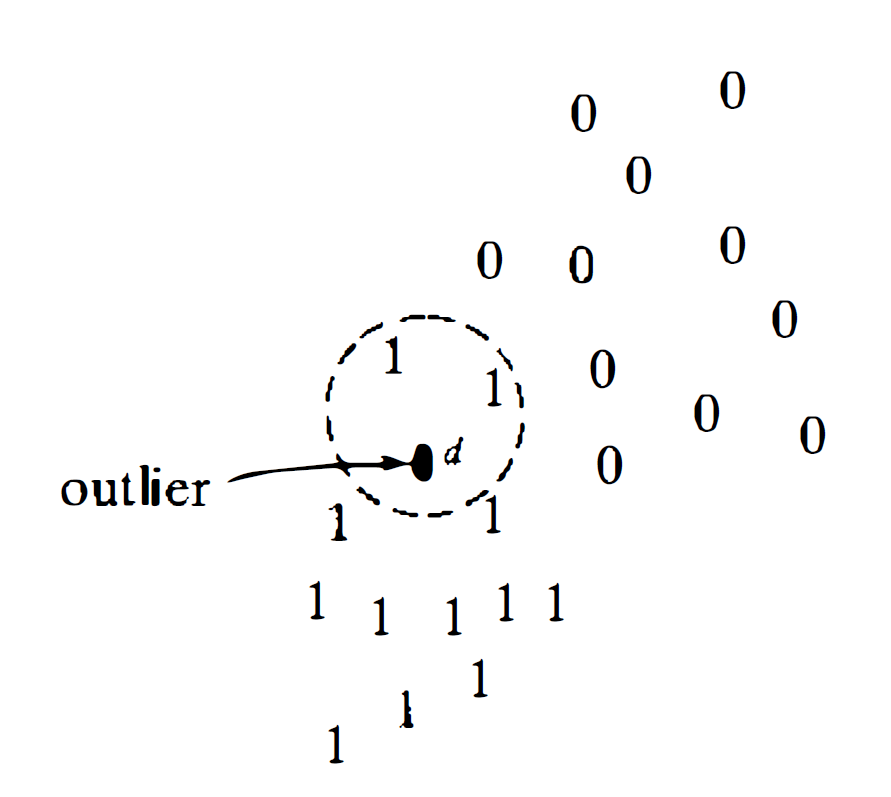
\includegraphics[width=0.4\textwidth]{Nearest.png}
  \caption{محدوده‌ی درون خطچین شامل دو نقطه متعلق به کلاس $1$ و یک داده‌ی پرت با مقدار $0$ است، الگوریتم $k$ نزدیک ترین همسایه $(k=3)$ مقدار  به طور شهودی صحیح $1$ را به نقطه‌ی $d$ نسبت می‌دهد، در حالی که $d$ به داده‌ی پرت $0$ نزدیک تر است.(کتاب شبکه های عصبی\cite[ص-55]{haykin}) }
  \label{fig:nearest}
\end{figure}

یک حالت دیگر از یادگیری‌های مبتنی بر حافظه که در واقع تعمیم روش قبل است، کلاس‌بندی $k$ نزدیک ترین همسایه است. در این روش همسایگی $\widehat x$، k آزمایشی است که در نزدیک ترین فاصله از بردار ورودی قرار دارند، و الگوریتم با یافتن کلاسی که در این $k$ آزمایش بیشتر از همه تکرار شده ، جواب مسئله را می‌دهد.\\


الگوریتم های دیگری نیز وجود دارند که بر پایه‌ی حافظه هستند اما ما به همین دو مورد بسنده می‌کنیم.\\

شکل \ref{fig:nearest} تفاوت این دو روش مبنی بر حافظه را نشان می‌دهد.

\subsection{بلتزمن (Boltzmann)}
\label{sec:boltzmann}
در سال ۱۹۸۶ هینتون و سجنوفسکی یک قانون یادگیری را برای شبکه‌های احتمالاتی متقارن ابداع کردند و نام آن را به خاطر توزیع بلتزمن به افتخار طراح آن نام گذاری کردند. به شبکه های عصبی‌ای که بر پایه‌ی این الگوریتم کار می‌کنند ماشین های بلتزمن (بخش 
\ref{sec:boltzmann_machine})
می‌گویند.

در یک ماشین بلتزمن هر عصب می‌تواند در $2$ حالت مختلف مثلا $+1$ یا $-1$ قرار گیرد و برای کل سیستم می‌توان یک تابع انرژی $E$ در نظر گرفت که مقدار آن با وضعیتی که عصب ها می‌گیرند تعیین می‌شود:
$$E=-\frac{1}{2} \underset{j \neq k}{\underset{j}{\sum} \underset{k}{\sum}} \omega_{kj} x_k x_j$$
ماشین در هر مرحله با انتخاب یک عصب تصادفی و عوض کردن وضعیت آن عصب با احتمالی که تابع زیر توصیف می‌کند در دمای $T$ تلاش می‌کند تا مقدار انرژی را به دمای تعادل برساند (البته که این دما کمیتی فیزیکی  نیست و می‌توان آن را شبه دما نامید).
$$P(x_k \rightarrow -x_k) = \frac{1}{1+\exp{(-\Delta E_k / T) }}$$
اینجا $\Delta E_k$ مقدار تغییرات انرژی بر اثر تغییر وضعیت عصب $k$ را نشان می‌دهد.\\
عصب های ماشین بلتزمن را می‌توان به دو دسته‌ی پنهان و آشکار تقسیم کرد، این ماشین در دو حالت مختلف عمل می کند:
\begin{enumerate}
\item
حالتی  که وضعیت عصب های آشکار از سوی محیط تحمیل می‌شود.
\item
حالتی که عصب های آشکار آزادانه تغییر می کنند.
\end{enumerate}
که در هر دو این حالات وضعیت عصب های پنهان به صورت آزاد می‌تواند تغییر کند. فرض کنید $\rho_{i,j}^{+}$ مقدار هم بستگی وضعیت های دو عصب $i$ و $j$  و میانگین گرفته شده درتمام وضعیت‌های تعادل حالت اول است. و $\rho_{i,j}^{-}$ همین هم بستگی در حالت دوم است. تغییر وزن اتصال بین این دو عصب را با فرمول زیر تعیین می‌کنیم:
$$\Delta \omega_{k,j} = \eta(\rho_{k,j}^{+} - \rho_{k,j}^{-}), \;\;\;\;\; j \neq k$$
که متغیر های بالا قبل تر تعریف شده اند. 
\subsection{هبین (Hebian)}
فرضیه‌ی هب یکی از قدیمی ترین و مشهور ترین قانون های یادگیری را ارائه می‌کند:

وقتی که یک عصب $A$ به اندازه کافی به عصب $B$ نزدیک باشد که آن را تحریک کند و به طور مداوم در فعال کردن عصب $B$ شرکت کند، فرایندی در یکی یا هر دو این عصب ها شکل می‌گیرد که تاثیر عصب $A$ را بر روی عصب $B$ افزایش می‌دهد. \cite[ص-۵۱]{haykin}

با عوض کردن جمله بندی این گزاره، دو قانون زیر را به دست می‌آوریم:
\begin{enumerate}
\item
اگر دو عصب در دو سمت یک سیناپس (یک اتصال) به طور هم‌زمان عمل کنند، در آن صورت قدرت آن سیناپس به دلخواهی افزایش می‌یابد.
\item
اگر دو عصب در دو سمت یک سیناپس (یک اتصال) به طور غیر هم زمان عمل کنند، در آن صورت قدرت آن سیناپس به دلخواهی کاهش می‌یابد. \cite[ص-۵۵]{haykin}
\end{enumerate}
به چنین سیناپسی سیناپس هبین می‌گویند، در واقع چنین اتصالی از یک فرایند فعال وابسته به زمان و به شدت موضعی برای بهبود کارایی عصب ها و بهینه سازی آنها استفاده می‌کند.

از تعریف اولیه، قانون دوم نوشته شده به دست نمی‌آید در واقع مدل های متفاوتی با توجه به قوانین هبین می‌توان ساخت که می‌توانند به صورت متفاوتی عمل کنند، برای مثال ممکن است تغییرات وزن اتصالات متناسب با حاصل ضرب وضعیت دو عصب تغییر کند که در این صورت سیناپس خاصیت کواریانسی پیدا می‌کند و یا این که تنها با هم‌زمانی ها تقویت شود و تضعیفی در کار نباشد که مشابه تعریف اولیه است.

به شباهت قوانین هبین با پدیده‌ی شرطی سازی در روانشناسی نیز می‌توان توجه کرد.

\subsection{آموزش رقابتی}
مشابه اسم این یادگیری، عصب های شبکه‌های عصبی در این روش با یکدیگر سر فعال شدن رقابت می‌کنند، برعکس روش های قبلی که در آن به طور هم‌زمان چند عصب از شبکه می‌توانستند فعالیت کنند، در این روش تنها عصب برنده فعال می‌شود، که این خاصیت این شبکه ها را برای کشف ویژگی های مهم آماری برای دسته بندی داده ها مناسب می‌سازد.
قواعد این روش را در سه عنصر می‌توان خلاصه کرد:
\begin{enumerate}
\item
یک مجموعه از عصب ها که کاملا مشابه اند، به جز در وزن اتصالات که به صورت تصادفی توزیع شده اند.
\item
یک محدودیت بر روی قدرت عصب ها.
\item
یک مکانیزم رقابت که عصب ها به وسیله‌ی آن بتوانند رقابت کنند و برنده تعیین شود.
\end{enumerate}
در ساده ترین حالت این شبکه می‌توان یک سطح از عصب های خروجی در نظر گرفت که همه‌ِی عصب های ورودی به همه‌ی آن‌ها اتصالاتی با وزن مثبت دارند (اتصالات بین عصب های خروجی نیز مشکلی ایجاد نمی‌کند).

برای این که عصب $k$ بین عصب ها برنده شود باید میدان القایی\LTRfootnote{Local induced field} آن به ازای ورودی $\widehat x$ در بین همه‌ی عصب ها بیشینه باشد، در نتیجه ورودی های عصب برنده به نحوی تغییر می‌کنند که عصب  $k$ با ورودی $\widehat x$ آموزش یابد و این عصب با این ورودی راحت تر تحریک شود، برای این کار بردار وزن اتصالات عصب $k$ به سمت ورودی $\widehat x$ شیفت داده می‌شود، یا به عبارتی:
$$\Delta \omega_{k,j}= \begin{cases} \eta(x_j-\omega_{k,j}) & \text{اگر عصب $k$ مسابقه را ببرد} \\ 0 & \text{اگر عصب $k$ مسابقه را ببازد}  \end{cases}$$
که ضریب $\eta$ همان ضریب یادگیری است. تعبیر شهودی فرایند ذکر شده این است که در صورت خوشه ای بودن داده ها در چند همسایگی، برای دسته بندی این داده ها به وسیله‌ی شبکه‌ی عصبی بالا در گروه‌های جدا از هم، می خواهیم که به هر گروه یک عصب نسبت دهیم که در صورتی که ورودی درون یکی از آن گروه ها فعال شود، عصب متناظر با آن گروه شروع به فعالیت کند. برای این کار بردار ورودی عصب ها را رندم در فضای حالات پراکنده می‌کنیم و در صورتی که بردار ورودی یک عصب به ورودی یک آزمایش نزدیک تر باشد(و در نتیجه بیشتر از بقیه‌ی عصب ها تحریک شود)، آن عصب را متناظر با گروه آن ورودی در نظر می‌گیریم و بردار آن را به بردار این ورودی نزدیک می‌کنیم. بعد از چندین مرحله اجرای این آزمایش به حالتی می‌رسیم که بردار هر عصب در میان گروه متناظر آن قرار دارد و در مراحل بعدی این عصب اعضای آن گروه را شناسایی می‌کند، از آن جا که بردار های ورودی در ابتدا تصادفی پراکنده شده بودند، به صورت احتمالی هر گروه یک عصب درون خود دارد، و از آنجا که هر آزمایش یک برنده دارد، در صورتی که یک گروه عصب متناظر خود را پیدا کند، از آن پس عصب برنده‌ی خود را خواهد داشت و بردار عصب های دیگر را به سمت خود نمی‌کشاند.



\begin{figure}
  \centering
    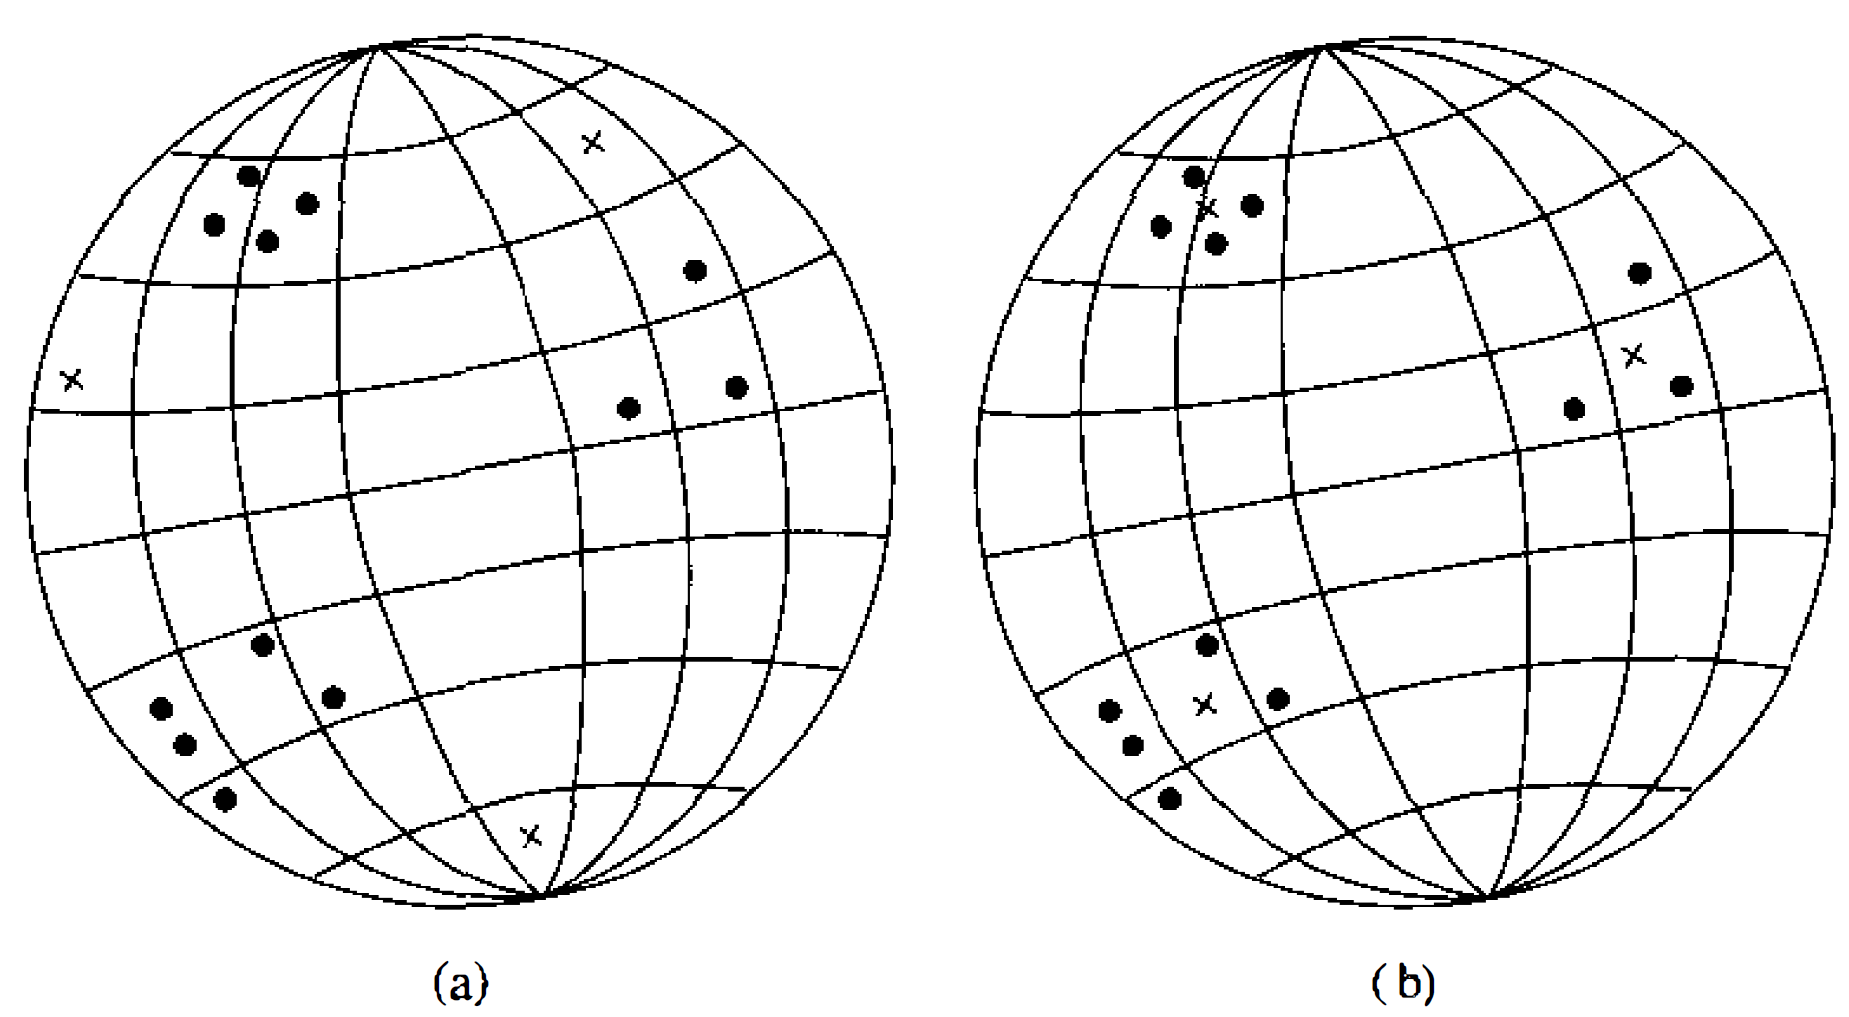
\includegraphics[width=0.4\textwidth]{competitive.png}
  \caption{فرایند یادگیری عصب ها در شبکه های رقابتی: شکل سمت چپ قبل از تحریک شدن توسط داده ها، شکل سمت راست بعد از تحریک شدن. هر یک از علامت های ضربدر نشان دهنده ی مکان یکی از بردارهای وزن اتصالات است، هر یک از نقطه ها نشان دهنده ی بردار ورودی یک داده است.(کتاب شبکه های عصبی\cite[ص-60]{haykin})}
  \label{fig:competitive}
\end{figure}
شکل \ref{fig:competitive} این فرایند را نشان می‌دهد.

\section{کاربرد‌های مهم}
در چند دهه‌ی اخیر بسیاری از فعالیت هایی که پیش از این تنها به وسیله‌ی انسان قابل انجام بوده، به وسیله‌ی کامپیوتر دست یافتنی شده است. علت این پیشرفت را می‌توان پیدایش پردازنده های قوی تر و همچنین الگوریتم های جدید ماشین‌لرنینگ  دانست.
به عنوان یکی از این الگوریتم ها شبکه‌های عصبی نیز نقش موثری در این فرایند داشته‌اند. مواردی که در ادامه مطرح می‌شود به طور کلی کاربرد هایی هستند که به وسیله‌ی شبکه های عصبی و یا سایر ماشین های یادگیری آماری ممکن شده اند.
\subsection{تشخیص الگو، صدا و تصویر}
امروزه پیشرفت ها در این زمینه تا حدی بوده که حتی بعضی از تلفن های همراه هم دارای امکاناتی همچون دستیار های صوتی و یا تشخیص چهره هستند، گرچه در ابتدا موفقیت های ماشین های آماری در این زمینه بسیار بیشتر از شبکه‌های عصبی بود ولی با پیدایش شبکه های عمیق و پیشرفت شبکه‌های عصبی، این شبکه‌ها از ماشین های آماری پیشی گرفتند.

در این مورد معرفی چند مورد مناسب به نظر می‌رسد:
\begin{enumerate}
\item
در الگوریتم‌های داده‌کاوی برای پیدا کردن الگوها و گشتن به دنبال بی‌قاعدگی‌ها به طور گسترده از شبکه‌های چند لایه (بخش
\ref{sec:multilayer})
استفاده می‌شود.
\item
برای پیدا کردن الگو مشابه در یک بانک از الگو‌ها می‌توان از شبکه‌های هاپفیلد (بخش 
\ref{sec:hopfield})
استفاده کرد.
\item
برای بازسازی عکس‌های آسیب‌دیده یا ناقص و یا بازیابی اطلاعات متون خطی که تا حدی از دست رفته‌اند می‌توانیم از شبکه‌های بلتزمن (بخش 
\ref{sec:boltzmann_machine})
یاری بجوییم.

\end{enumerate}

\subsection{خوشه‌سازی و دسته‌بندی}
وقتی حجم داده‌ها زیاد و یا تعداد ابعاد ورودی بیش 3 یا 4 بعد می‌شود ادراک انسان دچار مشکل شده و توانایی خود را در تجسم داده از دست می‌دهد، این مشکل برای کامپیوتر نیز به دلیل افزایش محاسبات به صورت نمایی با افزایش ابعاد ورودی وجود دارد اما شدت آن کم‌تر است.

الگوریتم‌های شبکه‌های عصبی تا به امروز در این کار بسیار موفق عمل کرده‌اند. در بعضی از این الگوریتم‌ها حتی نیاز به دانستن دسته‌بندی‌ها هم نیست (یادگیری بدون نظارت) و شبکه‌های عصبی تنها با داشتن ورودی‌های محتلف می‌توانند تا حد خوبی خصوصیات و ویژگی‌های مختلف داده‌ها را از یکدیگر تشخیص بدهند.

به عنوان مثال در این باره می‌توان شبکه‌های \lr{LSTM\LTRfootnote{Long Short-term Memory}} را نام برد که در سال ۲۰۰۹ برای تشخیص متن دست‌نوشت به کار رفت و مسابقه‌ی \lr{ICDAR} در همین زمینه را در سال مذکور از آن خود کرد.
\subsubsection{استخراج اطلاعات}
انسان ها در برابر حجم زیاد داده ها از ماشین ها عقب می مانند، علاوه بر این، گاهی ماشین ها نظمی در داده ها پیدا می‌کنند که انسان به طور شهودی قابلیت درک آن را ندارد. که باز هم می‌توان استفاده‌ی این الگوریتم‌ها در زمینه‌ی داده‌کاوی را خاطر نشان کرد.
\subsubsection{تحلیل اطلاعات}
 کامپیوتر ها در این زمینه هم ثابت کردند که در بعضی از موارد از انسان ها سریع ترند، بسیاری از شرکت های اقتصادی بر پایه‌ی این برنامه ها سرمایه‌گذاری های خود را انجام می‌دهند.
\subsection{بهینه‌سازی مسائل پیچیده}
مسائل NP دسته ای کاربردی از مسائل هستند که تا کنون الگوریتم ای قطعی برای حل آن ها در زمان مناسب ارائه نشده است. اما شبکه های عصبی و سایر ماشین‌های یادگیری می‌توانند آن ها را در زمان خیلی خوبی با اطمینان بالایی حل کنند. و شاید حتی این دسته از مسئله ها را بتوان علت این دانست که چرا الگوریتم های قطعی توانایی رقابت با مغز انسان را ندارند.
\subsection{سایر کاربردها}
چند نمونه از دیگر موارد کاربردی شبکه های عصبی:
\begin{enumerate}
\item
تقریب تابع‌ها:
تقریب زند توابعی که محاسبه ی آن ها به راحتی امکان پذیر نیست.
\item
پیش‌بینی و حدس:
پیشبینی وضع هوا، بازار، حدس زدن نتیجه‌ی یک رخداد و ....

البته تنوع کاربردی شبکه های عصبی بیشتر از مواردی که در اینجا بیان شده است.

\end{enumerate}

\begin{latin}
{
% سه دستور زیر باعث می‌شوند که مراجع با قلم کوچکتر و با فاصله خطوط کمتر و با فاصله بین مراجع کم ظاهر شوند.
% این حالت برای کاهش تعداد صفحات مقاله مناسب است.
% می‌توانید هر یک از آنها را comment نموده و خروجی را ملاحظه فرمایید.
\small
\singlespacing
\setlength{\itemsep}{-2ex}
%اگر از فایلهای سبک انگلیسی مانند latex8.bst یا ieeetr-fa استفاده کنید بایستی کل قسمت مراجع را در داخل یک محیط latin قرار دهید (که در حال حاضر comment شده است و دستور زیر را نیز از حالت comment خارج کنید.
\renewcommand{\refname}{\rl{{مراجع}\hfill}}
\bibliographystyle{ieeetr-fa}%{latex8}%{IEEEtrans}
%\bibliography{article}
\begin{thebibliography}{1}

    \bibitem{haykin}  S. Haykin, {\em Neural Networks: A Comprehensive Foundation}, 2\super{nd} ed., New Jersey, Prentice-Hall, 1999.
    
    \bibitem{russell}  S. J. Russell and P. Norvig, {\em Artificial Intelligence: A Modern Approach}, 3\super{rd} ed., New Jersey, Prentice-Hall, 2010
    \bibitem{bishop} C. M. Bishop, {\em Pattern Recognition and Machine Learning}, 1\super{st} ed., New York, Springer, 2006.
    

    \bibitem{ml-hinton}  G. Hinton, {\em Neural Networks and Machine Learning [lecture notes]}, Retrieved from coursera.org, 2012

    \bibitem{ml-andrew}  A. Ng, {\em Machine Learning [lecture notes]}. Retrieved from coursera.org, 2014
    
    \bibitem{hertz} J. Hertz, A. Krogh, R. G. Palmer, {\em Introduction to the theory of Neural Computation}, Lecture notes Volume I, California, Addison-Wesley publishing company, 1990.
    
    \bibitem{wiki-frank} Wikipedia contributors, "Frank Rosenblatt" {\em Wikipedia, The Free Encyclopedia}, [online], Available: {\em https://en.wikipedia.org/wiki/Frank\_Rosenblatt}
    
    \bibitem{wiki-overfitting} Wikipedia contributors, "Overfitting" {\em Wikipedia, The Free Encyclopedia}, [online], Available: {\em https://en.wikipedia.org/wiki/Overfitting}
    
    \bibitem{wiki-hopfield_net} Wikipedia contributors, "Hopfield network" {\em Wikipedia, The Free Encyclopedia}, [online], Available: {\em https://en.wikipedia.org/wiki/Hopfield\_network }

  \end{thebibliography}
}
\end{latin}

\end{document}
